\documentclass[1p]{elsarticle_modified}
%\bibliographystyle{elsarticle-num}

%\usepackage[colorlinks]{hyperref}
%\usepackage{abbrmath_seonhwa} %\Abb, \Ascr, \Acal ,\Abf, \Afrak
\usepackage{amsfonts}
\usepackage{amssymb}
\usepackage{amsmath}
\usepackage{amsthm}
\usepackage{scalefnt}
\usepackage{amsbsy}
\usepackage{kotex}
\usepackage{caption}
\usepackage{subfig}
\usepackage{color}
\usepackage{graphicx}
\usepackage{xcolor} %% white, black, red, green, blue, cyan, magenta, yellow
\usepackage{float}
\usepackage{setspace}
\usepackage{hyperref}

\usepackage{tikz}
\usetikzlibrary{arrows}

\usepackage{multirow}
\usepackage{array} % fixed length table
\usepackage{hhline}

%%%%%%%%%%%%%%%%%%%%%
\makeatletter
\renewcommand*\env@matrix[1][\arraystretch]{%
	\edef\arraystretch{#1}%
	\hskip -\arraycolsep
	\let\@ifnextchar\new@ifnextchar
	\array{*\c@MaxMatrixCols c}}
\makeatother %https://tex.stackexchange.com/questions/14071/how-can-i-increase-the-line-spacing-in-a-matrix
%%%%%%%%%%%%%%%

\usepackage[normalem]{ulem}

\newcommand{\msout}[1]{\ifmmode\text{\sout{\ensuremath{#1}}}\else\sout{#1}\fi}
%SOURCE: \msout is \stkout macro in https://tex.stackexchange.com/questions/20609/strikeout-in-math-mode

\newcommand{\cancel}[1]{
	\ifmmode
	{\color{red}\msout{#1}}
	\else
	{\color{red}\sout{#1}}
	\fi
}

\newcommand{\add}[1]{
	{\color{blue}\uwave{#1}}
}

\newcommand{\replace}[2]{
	\ifmmode
	{\color{red}\msout{#1}}{\color{blue}\uwave{#2}}
	\else
	{\color{red}\sout{#1}}{\color{blue}\uwave{#2}}
	\fi
}

\newcommand{\Sol}{\mathcal{S}} %segment
\newcommand{\D}{D} %diagram
\newcommand{\A}{\mathcal{A}} %arc


%%%%%%%%%%%%%%%%%%%%%%%%%%%%%5 test

\def\sl{\operatorname{\textup{SL}}(2,\Cbb)}
\def\psl{\operatorname{\textup{PSL}}(2,\Cbb)}
\def\quan{\mkern 1mu \triangleright \mkern 1mu}

\theoremstyle{definition}
\newtheorem{thm}{Theorem}[section]
\newtheorem{prop}[thm]{Proposition}
\newtheorem{lem}[thm]{Lemma}
\newtheorem{ques}[thm]{Question}
\newtheorem{cor}[thm]{Corollary}
\newtheorem{defn}[thm]{Definition}
\newtheorem{exam}[thm]{Example}
\newtheorem{rmk}[thm]{Remark}
\newtheorem{alg}[thm]{Algorithm}

\newcommand{\I}{\sqrt{-1}}
\begin{document}

%\begin{frontmatter}
%
%\title{Boundary parabolic representations of knots up to 8 crossings}
%
%%% Group authors per affiliation:
%\author{Yunhi Cho} 
%\address{Department of Mathematics, University of Seoul, Seoul, Korea}
%\ead{yhcho@uos.ac.kr}
%
%
%\author{Seonhwa Kim} %\fnref{s_kim}}
%\address{Center for Geometry and Physics, Institute for Basic Science, Pohang, 37673, Korea}
%\ead{ryeona17@ibs.re.kr}
%
%\author{Hyuk Kim}
%\address{Department of Mathematical Sciences, Seoul National University, Seoul 08826, Korea}
%\ead{hyukkim@snu.ac.kr}
%
%\author{Seokbeom Yoon}
%\address{Department of Mathematical Sciences, Seoul National University, Seoul, 08826,  Korea}
%\ead{sbyoon15@snu.ac.kr}
%
%\begin{abstract}
%We find all boundary parabolic representation of knots up to 8 crossings.
%
%\end{abstract}
%\begin{keyword}
%    \MSC[2010] 57M25 
%\end{keyword}
%
%\end{frontmatter}

%\linenumbers
%\tableofcontents
%
\newcommand\colored[1]{\textcolor{white}{\rule[-0.35ex]{0.8em}{1.4ex}}\kern-0.8em\color{red} #1}%
%\newcommand\colored[1]{\textcolor{white}{ #1}\kern-2.17ex	\textcolor{white}{ #1}\kern-1.81ex	\textcolor{white}{ #1}\kern-2.15ex\color{red}#1	}

{\Large $\underline{11a_{73}~(K11a_{73})}$}

\setlength{\tabcolsep}{10pt}
\renewcommand{\arraystretch}{1.6}
\vspace{1cm}\begin{tabular}{m{100pt}>{\centering\arraybackslash}m{274pt}}
\multirow{5}{120pt}{
	\centering
	\includegraphics[width=112pt]{../../../GIT/diagram.site/Diagrams/png/322_11a_73.png}\\
\ \ \ A knot diagram\footnotemark}&
\allowdisplaybreaks
\textbf{Linearized knot diagam} \\
\cline{2-2}
 &
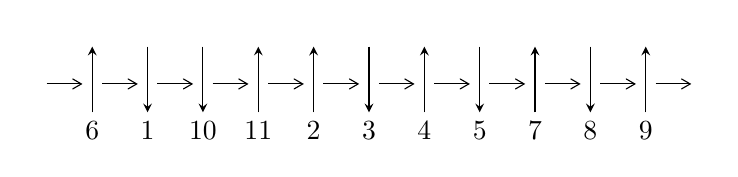
\begin{tikzpicture}[x=20pt, y=17pt]
	% nodes
	\node (C0) at (0, 0) {};
	\node (C1) at (1, 0) {};
	\node (C1U) at (1, +1) {};
	\node (C1D) at (1, -1) {6};

	\node (C2) at (2, 0) {};
	\node (C2U) at (2, +1) {};
	\node (C2D) at (2, -1) {1};

	\node (C3) at (3, 0) {};
	\node (C3U) at (3, +1) {};
	\node (C3D) at (3, -1) {10};

	\node (C4) at (4, 0) {};
	\node (C4U) at (4, +1) {};
	\node (C4D) at (4, -1) {11};

	\node (C5) at (5, 0) {};
	\node (C5U) at (5, +1) {};
	\node (C5D) at (5, -1) {2};

	\node (C6) at (6, 0) {};
	\node (C6U) at (6, +1) {};
	\node (C6D) at (6, -1) {3};

	\node (C7) at (7, 0) {};
	\node (C7U) at (7, +1) {};
	\node (C7D) at (7, -1) {4};

	\node (C8) at (8, 0) {};
	\node (C8U) at (8, +1) {};
	\node (C8D) at (8, -1) {5};

	\node (C9) at (9, 0) {};
	\node (C9U) at (9, +1) {};
	\node (C9D) at (9, -1) {7};

	\node (C10) at (10, 0) {};
	\node (C10U) at (10, +1) {};
	\node (C10D) at (10, -1) {8};

	\node (C11) at (11, 0) {};
	\node (C11U) at (11, +1) {};
	\node (C11D) at (11, -1) {9};
	\node (C12) at (12, 0) {};

	% arrows
	\draw[->,>={angle 60}]
	(C0) edge (C1) (C1) edge (C2) (C2) edge (C3) (C3) edge (C4) (C4) edge (C5) (C5) edge (C6) (C6) edge (C7) (C7) edge (C8) (C8) edge (C9) (C9) edge (C10) (C10) edge (C11) (C11) edge (C12) ;	\draw[->,>=stealth]
	(C1D) edge (C1U) (C2U) edge (C2D) (C3U) edge (C3D) (C4D) edge (C4U) (C5D) edge (C5U) (C6U) edge (C6D) (C7D) edge (C7U) (C8U) edge (C8D) (C9D) edge (C9U) (C10U) edge (C10D) (C11D) edge (C11U) ;
	\end{tikzpicture} \\
\hhline{~~} \\& 
\textbf{Solving Sequence} \\ \cline{2-2} 
 &
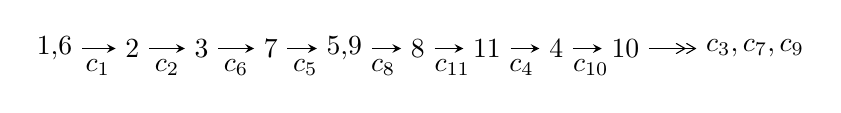
\begin{tikzpicture}[x=25pt, y=7pt]
	% node
	\node (A0) at (-1/8, 0) {1,6};
	\node (A1) at (1, 0) {2};
	\node (A2) at (2, 0) {3};
	\node (A3) at (3, 0) {7};
	\node (A4) at (65/16, 0) {5,9};
	\node (A5) at (41/8, 0) {8};
	\node (A6) at (49/8, 0) {11};
	\node (A7) at (57/8, 0) {4};
	\node (A8) at (65/8, 0) {10};
	\node (C1) at (1/2, -1) {$c_{1}$};
	\node (C2) at (3/2, -1) {$c_{2}$};
	\node (C3) at (5/2, -1) {$c_{6}$};
	\node (C4) at (7/2, -1) {$c_{5}$};
	\node (C5) at (37/8, -1) {$c_{8}$};
	\node (C6) at (45/8, -1) {$c_{11}$};
	\node (C7) at (53/8, -1) {$c_{4}$};
	\node (C8) at (61/8, -1) {$c_{10}$};
	\node (A9) at (10, 0) {$c_{3},c_{7},c_{9}$};

	% edge
	\draw[->,>=stealth]	
	(A0) edge (A1) (A1) edge (A2) (A2) edge (A3) (A3) edge (A4) (A4) edge (A5) (A5) edge (A6) (A6) edge (A7) (A7) edge (A8) ;
	\draw[->>,>={angle 60}]	
	(A8) edge (A9);
\end{tikzpicture} \\ 

\end{tabular} \\

\footnotetext{
The image of knot diagram is generated by the software ``\textbf{Draw programme}" developed by Andrew Bartholomew(\url{http://www.layer8.co.uk/maths/draw/index.htm\#Running-draw}), where we modified some parts for our purpose(\url{https://github.com/CATsTAILs/LinksPainter}).
}\phantom \\ \newline 
\centering \textbf{Ideals for irreducible components\footnotemark of $X_{\text{par}}$} 
 
\begin{align*}
I^u_{1}&=\langle 
-11711 u^{40}+64575 u^{39}+\cdots+3011 b-10581,\;-4430 u^{40}+27638 u^{39}+\cdots+3011 a-6831,\\
\phantom{I^u_{1}}&\phantom{= \langle  }u^{41}-6 u^{40}+\cdots+5 u-1\rangle \\
I^u_{2}&=\langle 
695 u^{30} a+2470 u^{30}+\cdots+1245 a-1088,\;4 u^{29} a- u^{30}+\cdots+6 a-2,\;u^{31}+2 u^{30}+\cdots+2 u+1\rangle \\
I^u_{3}&=\langle 
u^{11}+u^{10}+2 u^9+3 u^8+2 u^7+4 u^6+2 u^4- u^3+2 u^2+b-2 u+1,\\
\phantom{I^u_{3}}&\phantom{= \langle  }- u^{11}-4 u^9- u^8-6 u^7- u^6-4 u^5+u^4- u^3+3 u^2+a-1,\\
\phantom{I^u_{3}}&\phantom{= \langle  }u^{12}- u^{11}+4 u^{10}-3 u^9+7 u^8-5 u^7+7 u^6-6 u^5+6 u^4-6 u^3+4 u^2-2 u+1\rangle \\
I^u_{4}&=\langle 
b-1,\;a^2+2 a u+3 a+3 u+2,\;u^2+u+1\rangle \\
\\
I^v_{1}&=\langle 
a,\;b-1,\;v+1\rangle \\
\end{align*}
\raggedright * 5 irreducible components of $\dim_{\mathbb{C}}=0$, with total 120 representations.\\
\footnotetext{All coefficients of polynomials are rational numbers. But the coefficients are sometimes approximated in decimal forms when there is not enough margin.}
\newpage
\renewcommand{\arraystretch}{1}
\centering \section*{I. $I^u_{1}= \langle -11711 u^{40}+64575 u^{39}+\cdots+3011 b-10581,\;-4430 u^{40}+27638 u^{39}+\cdots+3011 a-6831,\;u^{41}-6 u^{40}+\cdots+5 u-1 \rangle$}
\flushleft \textbf{(i) Arc colorings}\\
\begin{tabular}{m{7pt} m{180pt} m{7pt} m{180pt} }
\flushright $a_{1}=$&$\begin{pmatrix}1\\0\end{pmatrix}$ \\
\flushright $a_{6}=$&$\begin{pmatrix}0\\u\end{pmatrix}$ \\
\flushright $a_{2}=$&$\begin{pmatrix}1\\- u^2\end{pmatrix}$ \\
\flushright $a_{3}=$&$\begin{pmatrix}u^2+1\\- u^2\end{pmatrix}$ \\
\flushright $a_{7}=$&$\begin{pmatrix}- u^5-2 u^3- u\\u^5+u^3+u\end{pmatrix}$ \\
\flushright $a_{5}=$&$\begin{pmatrix}- u\\u^3+u\end{pmatrix}$ \\
\flushright $a_{9}=$&$\begin{pmatrix}1.47127 u^{40}-9.17901 u^{39}+\cdots-5.53836 u+2.26868\\3.88941 u^{40}-21.4464 u^{39}+\cdots-12.0956 u+3.51411\end{pmatrix}$ \\
\flushright $a_{8}=$&$\begin{pmatrix}-0.531385 u^{40}-0.883427 u^{39}+\cdots-9.18931 u+3.76752\\6.82431 u^{40}-39.2046 u^{39}+\cdots-25.0438 u+5.73564\end{pmatrix}$ \\
\flushright $a_{11}=$&$\begin{pmatrix}-0.591498 u^{40}+4.05413 u^{39}+\cdots+5.08303 u+0.803720\\1.64198 u^{40}-9.67021 u^{39}+\cdots-8.71504 u+2.71837\end{pmatrix}$ \\
\flushright $a_{4}=$&$\begin{pmatrix}0.209565 u^{40}-0.0640983 u^{39}+\cdots+5.34341 u-3.59582\\1.85586 u^{40}-8.46463 u^{39}+\cdots+2.68615 u-1.43806\end{pmatrix}$ \\
\flushright $a_{10}=$&$\begin{pmatrix}5.73564 u^{40}-27.5895 u^{39}+\cdots-8.76918 u+3.63434\\-4.07174 u^{40}+21.9807 u^{39}+\cdots+6.42444 u-0.531385\end{pmatrix}$\\ \flushright $a_{10}=$&$\begin{pmatrix}5.73564 u^{40}-27.5895 u^{39}+\cdots-8.76918 u+3.63434\\-4.07174 u^{40}+21.9807 u^{39}+\cdots+6.42444 u-0.531385\end{pmatrix}$\\&\end{tabular}
\flushleft \textbf{(ii) Obstruction class $= -1$}\\~\\
\flushleft \textbf{(iii) Cusp Shapes $= -\frac{11684}{3011} u^{40}+\frac{62324}{3011} u^{39}+\cdots+\frac{34002}{3011} u+\frac{13707}{3011}$}\\~\\
\newpage\renewcommand{\arraystretch}{1}
\flushleft \textbf{(iv) u-Polynomials at the component}\newline \\
\begin{tabular}{m{50pt}|m{274pt}}
Crossings & \hspace{64pt}u-Polynomials at each crossing \\
\hline $$\begin{aligned}c_{1},c_{5}\end{aligned}$$&$\begin{aligned}
&u^{41}-6 u^{40}+\cdots+5 u-1
\end{aligned}$\\
\hline $$\begin{aligned}c_{2}\end{aligned}$$&$\begin{aligned}
&u^{41}+22 u^{40}+\cdots+11 u-1
\end{aligned}$\\
\hline $$\begin{aligned}c_{3},c_{8}\end{aligned}$$&$\begin{aligned}
&u^{41}+2 u^{40}+\cdots+8 u^2-1
\end{aligned}$\\
\hline $$\begin{aligned}c_{4},c_{7}\end{aligned}$$&$\begin{aligned}
&u^{41}+2 u^{40}+\cdots-24 u^2+1
\end{aligned}$\\
\hline $$\begin{aligned}c_{6}\end{aligned}$$&$\begin{aligned}
&u^{41}+6 u^{40}+\cdots-1163 u-157
\end{aligned}$\\
\hline $$\begin{aligned}c_{9},c_{11}\end{aligned}$$&$\begin{aligned}
&u^{41}-6 u^{40}+\cdots+4 u+1
\end{aligned}$\\
\hline $$\begin{aligned}c_{10}\end{aligned}$$&$\begin{aligned}
&u^{41}-22 u^{40}+\cdots+25 u^2-1
\end{aligned}$\\
\hline
\end{tabular}\\~\\
\newpage\renewcommand{\arraystretch}{1}
\flushleft \textbf{(v) Riley Polynomials at the component}\newline \\
\begin{tabular}{m{50pt}|m{274pt}}
Crossings & \hspace{64pt}Riley Polynomials at each crossing \\
\hline $$\begin{aligned}c_{1},c_{5}\end{aligned}$$&$\begin{aligned}
&y^{41}+22 y^{40}+\cdots+11 y-1
\end{aligned}$\\
\hline $$\begin{aligned}c_{2}\end{aligned}$$&$\begin{aligned}
&y^{41}-2 y^{40}+\cdots+119 y-1
\end{aligned}$\\
\hline $$\begin{aligned}c_{3},c_{8}\end{aligned}$$&$\begin{aligned}
&y^{41}-10 y^{40}+\cdots+16 y-1
\end{aligned}$\\
\hline $$\begin{aligned}c_{4},c_{7}\end{aligned}$$&$\begin{aligned}
&y^{41}-22 y^{40}+\cdots+48 y-1
\end{aligned}$\\
\hline $$\begin{aligned}c_{6}\end{aligned}$$&$\begin{aligned}
&y^{41}-20 y^{40}+\cdots+345571 y-24649
\end{aligned}$\\
\hline $$\begin{aligned}c_{9},c_{11}\end{aligned}$$&$\begin{aligned}
&y^{41}-14 y^{40}+\cdots+12 y-1
\end{aligned}$\\
\hline $$\begin{aligned}c_{10}\end{aligned}$$&$\begin{aligned}
&y^{41}+10 y^{39}+\cdots+50 y-1
\end{aligned}$\\
\hline
\end{tabular}\\~\\
\newpage\flushleft \textbf{(vi) Complex Volumes and Cusp Shapes}
$$\begin{array}{c|c|c}  
\text{Solutions to }I^u_{1}& \I (\text{vol} + \sqrt{-1}CS) & \text{Cusp shape}\\
 \hline 
\begin{aligned}
u &= \phantom{-}0.845612 + 0.498102 I \\
a &= \phantom{-}0.475474 + 0.261626 I \\
b &= -0.334988 - 0.050698 I\end{aligned}
 & \phantom{-}1.33190 + 2.47162 I & \phantom{-}16.2458 - 1.2870 I \\ \hline\begin{aligned}
u &= \phantom{-}0.845612 - 0.498102 I \\
a &= \phantom{-}0.475474 - 0.261626 I \\
b &= -0.334988 + 0.050698 I\end{aligned}
 & \phantom{-}1.33190 - 2.47162 I & \phantom{-}16.2458 + 1.2870 I \\ \hline\begin{aligned}
u &= -0.725875 + 0.718682 I \\
a &= \phantom{-}0.83857 + 1.21867 I \\
b &= -0.903416 - 0.468519 I\end{aligned}
 & \phantom{-}3.04955 + 5.79639 I & \phantom{-}4.67570 - 5.28890 I \\ \hline\begin{aligned}
u &= -0.725875 - 0.718682 I \\
a &= \phantom{-}0.83857 - 1.21867 I \\
b &= -0.903416 + 0.468519 I\end{aligned}
 & \phantom{-}3.04955 - 5.79639 I & \phantom{-}4.67570 + 5.28890 I \\ \hline\begin{aligned}
u &= -0.515395 + 0.785309 I \\
a &= -1.03703 - 1.54909 I \\
b &= \phantom{-}1.242510 + 0.373109 I\end{aligned}
 & \phantom{-}3.38107 - 0.44143 I & \phantom{-}9.27545 - 0.21018 I \\ \hline\begin{aligned}
u &= -0.515395 - 0.785309 I \\
a &= -1.03703 + 1.54909 I \\
b &= \phantom{-}1.242510 - 0.373109 I\end{aligned}
 & \phantom{-}3.38107 + 0.44143 I & \phantom{-}9.27545 + 0.21018 I \\ \hline\begin{aligned}
u &= -0.536686 + 0.762150 I \\
a &= -2.07413 - 0.35216 I \\
b &= \phantom{-}1.26360 - 0.68186 I\end{aligned}
 & \phantom{-}3.44275 - 3.84392 I & \phantom{-}9.44835 + 8.23646 I \\ \hline\begin{aligned}
u &= -0.536686 - 0.762150 I \\
a &= -2.07413 + 0.35216 I \\
b &= \phantom{-}1.26360 + 0.68186 I\end{aligned}
 & \phantom{-}3.44275 + 3.84392 I & \phantom{-}9.44835 - 8.23646 I \\ \hline\begin{aligned}
u &= -0.680543 + 0.851083 I \\
a &= \phantom{-}1.65602 + 0.00258 I \\
b &= -1.067800 + 0.649528 I\end{aligned}
 & \phantom{-}2.65853 - 11.08820 I & \phantom{-}3.28154 + 9.85902 I \\ \hline\begin{aligned}
u &= -0.680543 - 0.851083 I \\
a &= \phantom{-}1.65602 - 0.00258 I \\
b &= -1.067800 - 0.649528 I\end{aligned}
 & \phantom{-}2.65853 + 11.08820 I & \phantom{-}3.28154 - 9.85902 I\\
 \hline 
 \end{array}$$\newpage$$\begin{array}{c|c|c}  
\text{Solutions to }I^u_{1}& \I (\text{vol} + \sqrt{-1}CS) & \text{Cusp shape}\\
 \hline 
\begin{aligned}
u &= \phantom{-}0.193943 + 0.889112 I \\
a &= \phantom{-}0.883549 + 0.178964 I \\
b &= \phantom{-}0.138077 + 0.486291 I\end{aligned}
 & -0.85333 + 1.82668 I & -2.01304 - 4.52189 I \\ \hline\begin{aligned}
u &= \phantom{-}0.193943 - 0.889112 I \\
a &= \phantom{-}0.883549 - 0.178964 I \\
b &= \phantom{-}0.138077 - 0.486291 I\end{aligned}
 & -0.85333 - 1.82668 I & -2.01304 + 4.52189 I \\ \hline\begin{aligned}
u &= \phantom{-}0.857936 + 0.229320 I \\
a &= \phantom{-}1.55370 - 0.62249 I \\
b &= -1.20325 + 1.09295 I\end{aligned}
 & -0.91359 - 13.22010 I & \phantom{-}1.63608 + 7.45702 I \\ \hline\begin{aligned}
u &= \phantom{-}0.857936 - 0.229320 I \\
a &= \phantom{-}1.55370 + 0.62249 I \\
b &= -1.20325 - 1.09295 I\end{aligned}
 & -0.91359 + 13.22010 I & \phantom{-}1.63608 - 7.45702 I \\ \hline\begin{aligned}
u &= \phantom{-}0.848782\phantom{ +0.000000I} \\
a &= -0.709994\phantom{ +0.000000I} \\
b &= \phantom{-}0.892393\phantom{ +0.000000I}\end{aligned}
 & \phantom{-}0.744100\phantom{ +0.000000I} & \phantom{-}9.40900\phantom{ +0.000000I} \\ \hline\begin{aligned}
u &= \phantom{-}0.454786 + 1.065100 I \\
a &= -0.31016 + 1.42726 I \\
b &= \phantom{-}0.511379 + 0.571103 I\end{aligned}
 & -0.42808 + 3.78436 I & \phantom{-}2.16188 - 5.53774 I \\ \hline\begin{aligned}
u &= \phantom{-}0.454786 - 1.065100 I \\
a &= -0.31016 - 1.42726 I \\
b &= \phantom{-}0.511379 - 0.571103 I\end{aligned}
 & -0.42808 - 3.78436 I & \phantom{-}2.16188 + 5.53774 I \\ \hline\begin{aligned}
u &= \phantom{-}0.539684 + 1.034030 I \\
a &= \phantom{-}0.779420 - 0.504456 I \\
b &= -0.164278 - 0.300558 I\end{aligned}
 & -0.14735 + 2.61609 I & \phantom{-}2.94577 - 3.55552 I \\ \hline\begin{aligned}
u &= \phantom{-}0.539684 - 1.034030 I \\
a &= \phantom{-}0.779420 + 0.504456 I \\
b &= -0.164278 + 0.300558 I\end{aligned}
 & -0.14735 - 2.61609 I & \phantom{-}2.94577 + 3.55552 I \\ \hline\begin{aligned}
u &= -0.455367 + 1.107240 I \\
a &= -1.04912 - 1.13395 I \\
b &= \phantom{-}1.50116 + 0.16642 I\end{aligned}
 & -0.93408 - 3.72501 I & \phantom{-0.000000 -}0. + 3.78091 I\\
 \hline 
 \end{array}$$\newpage$$\begin{array}{c|c|c}  
\text{Solutions to }I^u_{1}& \I (\text{vol} + \sqrt{-1}CS) & \text{Cusp shape}\\
 \hline 
\begin{aligned}
u &= -0.455367 - 1.107240 I \\
a &= -1.04912 + 1.13395 I \\
b &= \phantom{-}1.50116 - 0.16642 I\end{aligned}
 & -0.93408 + 3.72501 I & \phantom{-0.000000 } 0. - 3.78091 I \\ \hline\begin{aligned}
u &= \phantom{-}0.362831 + 1.165210 I \\
a &= \phantom{-}1.070360 - 0.324888 I \\
b &= \phantom{-}0.79605 - 1.29861 I\end{aligned}
 & -2.85882 - 1.02122 I & \phantom{-0.000000 } 0 \\ \hline\begin{aligned}
u &= \phantom{-}0.362831 - 1.165210 I \\
a &= \phantom{-}1.070360 + 0.324888 I \\
b &= \phantom{-}0.79605 + 1.29861 I\end{aligned}
 & -2.85882 + 1.02122 I & \phantom{-0.000000 } 0 \\ \hline\begin{aligned}
u &= \phantom{-}0.746103 + 0.183057 I \\
a &= -1.285710 + 0.387657 I \\
b &= \phantom{-}1.07761 - 1.20252 I\end{aligned}
 & \phantom{-}1.05085 - 4.60926 I & \phantom{-}7.98736 + 6.22230 I \\ \hline\begin{aligned}
u &= \phantom{-}0.746103 - 0.183057 I \\
a &= -1.285710 - 0.387657 I \\
b &= \phantom{-}1.07761 + 1.20252 I\end{aligned}
 & \phantom{-}1.05085 + 4.60926 I & \phantom{-}7.98736 - 6.22230 I \\ \hline\begin{aligned}
u &= -0.448486 + 1.175510 I \\
a &= \phantom{-}0.492889 + 0.632416 I \\
b &= -0.817436 - 0.184411 I\end{aligned}
 & -5.68068 - 4.22254 I & \phantom{-0.000000 } 0 \\ \hline\begin{aligned}
u &= -0.448486 - 1.175510 I \\
a &= \phantom{-}0.492889 - 0.632416 I \\
b &= -0.817436 + 0.184411 I\end{aligned}
 & -5.68068 + 4.22254 I & \phantom{-0.000000 } 0 \\ \hline\begin{aligned}
u &= \phantom{-}0.514268 + 1.164380 I \\
a &= -1.64613 + 1.51432 I \\
b &= \phantom{-}1.15140 + 1.37689 I\end{aligned}
 & -1.79982 + 9.32852 I & \phantom{-0.000000 } 0 \\ \hline\begin{aligned}
u &= \phantom{-}0.514268 - 1.164380 I \\
a &= -1.64613 - 1.51432 I \\
b &= \phantom{-}1.15140 - 1.37689 I\end{aligned}
 & -1.79982 - 9.32852 I & \phantom{-0.000000 } 0 \\ \hline\begin{aligned}
u &= \phantom{-}0.297512 + 1.244050 I \\
a &= -0.449120 + 0.044426 I \\
b &= -1.03032 + 1.16487 I\end{aligned}
 & -5.61358 - 9.45917 I & \phantom{-0.000000 } 0\\
 \hline 
 \end{array}$$\newpage$$\begin{array}{c|c|c}  
\text{Solutions to }I^u_{1}& \I (\text{vol} + \sqrt{-1}CS) & \text{Cusp shape}\\
 \hline 
\begin{aligned}
u &= \phantom{-}0.297512 - 1.244050 I \\
a &= -0.449120 - 0.044426 I \\
b &= -1.03032 - 1.16487 I\end{aligned}
 & -5.61358 + 9.45917 I & \phantom{-0.000000 } 0 \\ \hline\begin{aligned}
u &= -0.717723\phantom{ +0.000000I} \\
a &= \phantom{-}1.31735\phantom{ +0.000000I} \\
b &= -0.635831\phantom{ +0.000000I}\end{aligned}
 & -2.35187\phantom{ +0.000000I} & -3.23270\phantom{ +0.000000I} \\ \hline\begin{aligned}
u &= \phantom{-}0.559000 + 1.189400 I \\
a &= \phantom{-}1.71865 - 1.26258 I \\
b &= -1.27637 - 1.18033 I\end{aligned}
 & -3.7858 + 18.4184 I & \phantom{-0.000000 } 0 \\ \hline\begin{aligned}
u &= \phantom{-}0.559000 - 1.189400 I \\
a &= \phantom{-}1.71865 + 1.26258 I \\
b &= -1.27637 + 1.18033 I\end{aligned}
 & -3.7858 - 18.4184 I & \phantom{-0.000000 } 0 \\ \hline\begin{aligned}
u &= \phantom{-}0.220242 + 1.309270 I \\
a &= \phantom{-}0.00788396 - 0.00223172 I \\
b &= -0.246595 - 0.581812 I\end{aligned}
 & -4.69336 + 5.76085 I & \phantom{-0.000000 } 0 \\ \hline\begin{aligned}
u &= \phantom{-}0.220242 - 1.309270 I \\
a &= \phantom{-}0.00788396 + 0.00223172 I \\
b &= -0.246595 + 0.581812 I\end{aligned}
 & -4.69336 - 5.76085 I & \phantom{-0.000000 } 0 \\ \hline\begin{aligned}
u &= \phantom{-}0.506994 + 1.237050 I \\
a &= -0.343128 + 0.730701 I \\
b &= \phantom{-}0.837607 + 0.284107 I\end{aligned}
 & -2.86146 + 4.86399 I & \phantom{-0.000000 } 0 \\ \hline\begin{aligned}
u &= \phantom{-}0.506994 - 1.237050 I \\
a &= -0.343128 - 0.730701 I \\
b &= \phantom{-}0.837607 - 0.284107 I\end{aligned}
 & -2.86146 - 4.86399 I & \phantom{-0.000000 } 0 \\ \hline\begin{aligned}
u &= \phantom{-}0.337324 + 0.271834 I \\
a &= -0.07427 - 1.63066 I \\
b &= \phantom{-}0.823540 - 0.201797 I\end{aligned}
 & \phantom{-}1.65904 - 0.03957 I & \phantom{-}6.61397 + 0.60191 I \\ \hline\begin{aligned}
u &= \phantom{-}0.337324 - 0.271834 I \\
a &= -0.07427 + 1.63066 I \\
b &= \phantom{-}0.823540 + 0.201797 I\end{aligned}
 & \phantom{-}1.65904 + 0.03957 I & \phantom{-}6.61397 - 0.60191 I\\
 \hline 
 \end{array}$$\newpage$$\begin{array}{c|c|c}  
\text{Solutions to }I^u_{1}& \I (\text{vol} + \sqrt{-1}CS) & \text{Cusp shape}\\
 \hline 
\begin{aligned}
u &= -0.278824\phantom{ +0.000000I} \\
a &= -5.02278\phantom{ +0.000000I} \\
b &= \phantom{-}1.14650\phantom{ +0.000000I}\end{aligned}
 & \phantom{-}1.63641\phantom{ +0.000000I} & \phantom{-}6.23630\phantom{ +0.000000I}\\
 \hline 
 \end{array}$$\newpage\newpage\renewcommand{\arraystretch}{1}
\centering \section*{II. $I^u_{2}= \langle 695 u^{30} a+2470 u^{30}+\cdots+1245 a-1088,\;4 u^{29} a- u^{30}+\cdots+6 a-2,\;u^{31}+2 u^{30}+\cdots+2 u+1 \rangle$}
\flushleft \textbf{(i) Arc colorings}\\
\begin{tabular}{m{7pt} m{180pt} m{7pt} m{180pt} }
\flushright $a_{1}=$&$\begin{pmatrix}1\\0\end{pmatrix}$ \\
\flushright $a_{6}=$&$\begin{pmatrix}0\\u\end{pmatrix}$ \\
\flushright $a_{2}=$&$\begin{pmatrix}1\\- u^2\end{pmatrix}$ \\
\flushright $a_{3}=$&$\begin{pmatrix}u^2+1\\- u^2\end{pmatrix}$ \\
\flushright $a_{7}=$&$\begin{pmatrix}- u^5-2 u^3- u\\u^5+u^3+u\end{pmatrix}$ \\
\flushright $a_{5}=$&$\begin{pmatrix}- u\\u^3+u\end{pmatrix}$ \\
\flushright $a_{9}=$&$\begin{pmatrix}a\\-0.622202 a u^{30}-2.21128 u^{30}+\cdots-1.11459 a+0.974038\end{pmatrix}$ \\
\flushright $a_{8}=$&$\begin{pmatrix}-0.209490 a u^{30}+0.780662 u^{30}+\cdots+0.660698 a-1.61594\\-0.339302 a u^{30}-3.61594 u^{30}+\cdots-0.622202 a+0.788720\end{pmatrix}$ \\
\flushright $a_{11}=$&$\begin{pmatrix}-0.788720 a u^{30}-0.795882 u^{30}+\cdots+0.0259624 a+3.27932\\-1.01253 a u^{30}+2.10654 u^{30}+\cdots-0.806625 a-1.64369\end{pmatrix}$ \\
\flushright $a_{4}=$&$\begin{pmatrix}-2.04118 a u^{30}+3.35004 u^{30}+\cdots-1.79320 a+1.74217\\0.509400 a u^{30}-0.829902 u^{30}+\cdots+1.85497 a+1.23277\end{pmatrix}$ \\
\flushright $a_{10}=$&$\begin{pmatrix}-0.622202 a u^{30}+0.788720 u^{30}+\cdots-0.114593 a+0.974038\\-0.153089 a u^{30}-3.19875 u^{30}+\cdots-0.209490 a-0.219338\end{pmatrix}$\\ \flushright $a_{10}=$&$\begin{pmatrix}-0.622202 a u^{30}+0.788720 u^{30}+\cdots-0.114593 a+0.974038\\-0.153089 a u^{30}-3.19875 u^{30}+\cdots-0.209490 a-0.219338\end{pmatrix}$\\&\end{tabular}
\flushleft \textbf{(ii) Obstruction class $= -1$}\\~\\
\flushleft \textbf{(iii) Cusp Shapes $= 9 u^{30}+12 u^{29}+79 u^{28}+93 u^{27}+328 u^{26}+374 u^{25}+861 u^{24}+990 u^{23}+1590 u^{22}+1876 u^{21}+2214 u^{20}+2605 u^{19}+2432 u^{18}+2616 u^{17}+2165 u^{16}+1828 u^{15}+1490 u^{14}+816 u^{13}+642 u^{12}+206 u^{11}-4 u^9-174 u^8-52 u^7-60 u^6-64 u^5+4 u^4-7 u^3+12 u^2+16 u-1$}\\~\\
\newpage\renewcommand{\arraystretch}{1}
\flushleft \textbf{(iv) u-Polynomials at the component}\newline \\
\begin{tabular}{m{50pt}|m{274pt}}
Crossings & \hspace{64pt}u-Polynomials at each crossing \\
\hline $$\begin{aligned}c_{1},c_{5}\end{aligned}$$&$\begin{aligned}
&(u^{31}+2 u^{30}+\cdots+2 u+1)^{2}
\end{aligned}$\\
\hline $$\begin{aligned}c_{2}\end{aligned}$$&$\begin{aligned}
&(u^{31}+16 u^{30}+\cdots-2 u-1)^{2}
\end{aligned}$\\
\hline $$\begin{aligned}c_{3},c_{8}\end{aligned}$$&$\begin{aligned}
&u^{62}-4 u^{60}+\cdots-391 u+173
\end{aligned}$\\
\hline $$\begin{aligned}c_{4},c_{7}\end{aligned}$$&$\begin{aligned}
&u^{62}+6 u^{60}+\cdots- u+1
\end{aligned}$\\
\hline $$\begin{aligned}c_{6}\end{aligned}$$&$\begin{aligned}
&(u^{31}-2 u^{30}+\cdots-26 u+5)^{2}
\end{aligned}$\\
\hline $$\begin{aligned}c_{9},c_{11}\end{aligned}$$&$\begin{aligned}
&u^{62}+5 u^{61}+\cdots+30 u+1
\end{aligned}$\\
\hline $$\begin{aligned}c_{10}\end{aligned}$$&$\begin{aligned}
&(u^{31}+15 u^{30}+\cdots+6 u+4)^{2}
\end{aligned}$\\
\hline
\end{tabular}\\~\\
\newpage\renewcommand{\arraystretch}{1}
\flushleft \textbf{(v) Riley Polynomials at the component}\newline \\
\begin{tabular}{m{50pt}|m{274pt}}
Crossings & \hspace{64pt}Riley Polynomials at each crossing \\
\hline $$\begin{aligned}c_{1},c_{5}\end{aligned}$$&$\begin{aligned}
&(y^{31}+16 y^{30}+\cdots-2 y-1)^{2}
\end{aligned}$\\
\hline $$\begin{aligned}c_{2}\end{aligned}$$&$\begin{aligned}
&(y^{31}+32 y^{29}+\cdots+14 y-1)^{2}
\end{aligned}$\\
\hline $$\begin{aligned}c_{3},c_{8}\end{aligned}$$&$\begin{aligned}
&y^{62}-8 y^{61}+\cdots-1236207 y+29929
\end{aligned}$\\
\hline $$\begin{aligned}c_{4},c_{7}\end{aligned}$$&$\begin{aligned}
&y^{62}+12 y^{61}+\cdots-47 y+1
\end{aligned}$\\
\hline $$\begin{aligned}c_{6}\end{aligned}$$&$\begin{aligned}
&(y^{31}-16 y^{30}+\cdots-534 y-25)^{2}
\end{aligned}$\\
\hline $$\begin{aligned}c_{9},c_{11}\end{aligned}$$&$\begin{aligned}
&y^{62}+23 y^{61}+\cdots-104 y+1
\end{aligned}$\\
\hline $$\begin{aligned}c_{10}\end{aligned}$$&$\begin{aligned}
&(y^{31}-5 y^{30}+\cdots+236 y-16)^{2}
\end{aligned}$\\
\hline
\end{tabular}\\~\\
\newpage\flushleft \textbf{(vi) Complex Volumes and Cusp Shapes}
$$\begin{array}{c|c|c}  
\text{Solutions to }I^u_{2}& \I (\text{vol} + \sqrt{-1}CS) & \text{Cusp shape}\\
 \hline 
\begin{aligned}
u &= \phantom{-}0.700328 + 0.800493 I \\
a &= \phantom{-}1.146060 - 0.099237 I \\
b &= -0.574058 - 0.237024 I\end{aligned}
 & \phantom{-}0.66027 + 2.65228 I & -9.42163 - 5.74104 I \\ \hline\begin{aligned}
u &= \phantom{-}0.700328 + 0.800493 I \\
a &= -0.261910 - 0.128100 I \\
b &= \phantom{-}0.301124 + 0.295589 I\end{aligned}
 & \phantom{-}0.66027 + 2.65228 I & -9.42163 - 5.74104 I \\ \hline\begin{aligned}
u &= \phantom{-}0.700328 - 0.800493 I \\
a &= \phantom{-}1.146060 + 0.099237 I \\
b &= -0.574058 + 0.237024 I\end{aligned}
 & \phantom{-}0.66027 - 2.65228 I & -9.42163 + 5.74104 I \\ \hline\begin{aligned}
u &= \phantom{-}0.700328 - 0.800493 I \\
a &= -0.261910 + 0.128100 I \\
b &= \phantom{-}0.301124 - 0.295589 I\end{aligned}
 & \phantom{-}0.66027 - 2.65228 I & -9.42163 + 5.74104 I \\ \hline\begin{aligned}
u &= \phantom{-}0.576719 + 0.939494 I \\
a &= \phantom{-}0.06205 + 1.48991 I \\
b &= \phantom{-}0.971416 - 0.435463 I\end{aligned}
 & \phantom{-}1.79992 + 1.42306 I & \phantom{-}5.96720 + 7.06639 I \\ \hline\begin{aligned}
u &= \phantom{-}0.576719 + 0.939494 I \\
a &= \phantom{-}1.56139 - 0.38632 I \\
b &= -0.912307 + 0.063353 I\end{aligned}
 & \phantom{-}1.79992 + 1.42306 I & \phantom{-}5.96720 + 7.06639 I \\ \hline\begin{aligned}
u &= \phantom{-}0.576719 - 0.939494 I \\
a &= \phantom{-}0.06205 - 1.48991 I \\
b &= \phantom{-}0.971416 + 0.435463 I\end{aligned}
 & \phantom{-}1.79992 - 1.42306 I & \phantom{-}5.96720 - 7.06639 I \\ \hline\begin{aligned}
u &= \phantom{-}0.576719 - 0.939494 I \\
a &= \phantom{-}1.56139 + 0.38632 I \\
b &= -0.912307 - 0.063353 I\end{aligned}
 & \phantom{-}1.79992 - 1.42306 I & \phantom{-}5.96720 - 7.06639 I \\ \hline\begin{aligned}
u &= -0.847519 + 0.248601 I \\
a &= -0.626669 - 0.783073 I \\
b &= \phantom{-}0.478939 + 1.042720 I\end{aligned}
 & -2.48415 + 4.99236 I & -3.07968 - 5.91781 I \\ \hline\begin{aligned}
u &= -0.847519 + 0.248601 I \\
a &= \phantom{-}1.43877 + 0.44457 I \\
b &= -0.893298 - 0.771257 I\end{aligned}
 & -2.48415 + 4.99236 I & -3.07968 - 5.91781 I\\
 \hline 
 \end{array}$$\newpage$$\begin{array}{c|c|c}  
\text{Solutions to }I^u_{2}& \I (\text{vol} + \sqrt{-1}CS) & \text{Cusp shape}\\
 \hline 
\begin{aligned}
u &= -0.847519 - 0.248601 I \\
a &= -0.626669 + 0.783073 I \\
b &= \phantom{-}0.478939 - 1.042720 I\end{aligned}
 & -2.48415 - 4.99236 I & -3.07968 + 5.91781 I \\ \hline\begin{aligned}
u &= -0.847519 - 0.248601 I \\
a &= \phantom{-}1.43877 - 0.44457 I \\
b &= -0.893298 + 0.771257 I\end{aligned}
 & -2.48415 - 4.99236 I & -3.07968 + 5.91781 I \\ \hline\begin{aligned}
u &= \phantom{-}0.613097 + 0.623277 I \\
a &= -1.44473 - 0.64813 I \\
b &= \phantom{-}1.074650 + 0.709661 I\end{aligned}
 & \phantom{-}2.71352 + 3.26681 I & \phantom{-}9.13719 - 8.60586 I \\ \hline\begin{aligned}
u &= \phantom{-}0.613097 + 0.623277 I \\
a &= \phantom{-}1.88374 - 1.08780 I \\
b &= -0.810431 - 0.123872 I\end{aligned}
 & \phantom{-}2.71352 + 3.26681 I & \phantom{-}9.13719 - 8.60586 I \\ \hline\begin{aligned}
u &= \phantom{-}0.613097 - 0.623277 I \\
a &= -1.44473 + 0.64813 I \\
b &= \phantom{-}1.074650 - 0.709661 I\end{aligned}
 & \phantom{-}2.71352 - 3.26681 I & \phantom{-}9.13719 + 8.60586 I \\ \hline\begin{aligned}
u &= \phantom{-}0.613097 - 0.623277 I \\
a &= \phantom{-}1.88374 + 1.08780 I \\
b &= -0.810431 + 0.123872 I\end{aligned}
 & \phantom{-}2.71352 - 3.26681 I & \phantom{-}9.13719 + 8.60586 I \\ \hline\begin{aligned}
u &= -0.358609 + 1.074610 I \\
a &= \phantom{-}1.247210 + 0.063972 I \\
b &= \phantom{-}0.74515 + 1.66291 I\end{aligned}
 & -2.29804 + 2.01394 I & \phantom{-}0.79058 - 3.76194 I \\ \hline\begin{aligned}
u &= -0.358609 + 1.074610 I \\
a &= -0.49075 - 1.65979 I \\
b &= -0.0812528 - 0.0525556 I\end{aligned}
 & -2.29804 + 2.01394 I & \phantom{-}0.79058 - 3.76194 I \\ \hline\begin{aligned}
u &= -0.358609 - 1.074610 I \\
a &= \phantom{-}1.247210 - 0.063972 I \\
b &= \phantom{-}0.74515 - 1.66291 I\end{aligned}
 & -2.29804 - 2.01394 I & \phantom{-}0.79058 + 3.76194 I \\ \hline\begin{aligned}
u &= -0.358609 - 1.074610 I \\
a &= -0.49075 + 1.65979 I \\
b &= -0.0812528 + 0.0525556 I\end{aligned}
 & -2.29804 - 2.01394 I & \phantom{-}0.79058 + 3.76194 I\\
 \hline 
 \end{array}$$\newpage$$\begin{array}{c|c|c}  
\text{Solutions to }I^u_{2}& \I (\text{vol} + \sqrt{-1}CS) & \text{Cusp shape}\\
 \hline 
\begin{aligned}
u &= -0.066980 + 0.843210 I \\
a &= \phantom{-}0.905300 + 1.065700 I \\
b &= \phantom{-}0.372827 + 1.045040 I\end{aligned}
 & -1.82841 + 2.63278 I & -4.56232 - 0.80559 I \\ \hline\begin{aligned}
u &= -0.066980 + 0.843210 I \\
a &= \phantom{-}1.50981 - 0.90367 I \\
b &= -0.830677 + 0.572923 I\end{aligned}
 & -1.82841 + 2.63278 I & -4.56232 - 0.80559 I \\ \hline\begin{aligned}
u &= -0.066980 - 0.843210 I \\
a &= \phantom{-}0.905300 - 1.065700 I \\
b &= \phantom{-}0.372827 - 1.045040 I\end{aligned}
 & -1.82841 - 2.63278 I & -4.56232 + 0.80559 I \\ \hline\begin{aligned}
u &= -0.066980 - 0.843210 I \\
a &= \phantom{-}1.50981 + 0.90367 I \\
b &= -0.830677 - 0.572923 I\end{aligned}
 & -1.82841 - 2.63278 I & -4.56232 + 0.80559 I \\ \hline\begin{aligned}
u &= \phantom{-}0.423601 + 1.144370 I \\
a &= \phantom{-}0.200693 - 0.558634 I \\
b &= \phantom{-}0.664215 - 1.092670 I\end{aligned}
 & -5.31357 - 0.42431 I & -6.76845 + 0.89097 I \\ \hline\begin{aligned}
u &= \phantom{-}0.423601 + 1.144370 I \\
a &= \phantom{-}1.84585 - 1.43049 I \\
b &= -1.19733 - 1.54730 I\end{aligned}
 & -5.31357 - 0.42431 I & -6.76845 + 0.89097 I \\ \hline\begin{aligned}
u &= \phantom{-}0.423601 - 1.144370 I \\
a &= \phantom{-}0.200693 + 0.558634 I \\
b &= \phantom{-}0.664215 + 1.092670 I\end{aligned}
 & -5.31357 + 0.42431 I & -6.76845 - 0.89097 I \\ \hline\begin{aligned}
u &= \phantom{-}0.423601 - 1.144370 I \\
a &= \phantom{-}1.84585 + 1.43049 I \\
b &= -1.19733 + 1.54730 I\end{aligned}
 & -5.31357 + 0.42431 I & -6.76845 - 0.89097 I \\ \hline\begin{aligned}
u &= \phantom{-}0.470485 + 1.145180 I \\
a &= -1.312440 - 0.512271 I \\
b &= -0.95000 + 1.91169 I\end{aligned}
 & -4.97995 + 8.43248 I & -5.41543 - 9.16645 I \\ \hline\begin{aligned}
u &= \phantom{-}0.470485 + 1.145180 I \\
a &= -2.00403 + 1.37416 I \\
b &= \phantom{-}0.787153 + 0.878249 I\end{aligned}
 & -4.97995 + 8.43248 I & -5.41543 - 9.16645 I\\
 \hline 
 \end{array}$$\newpage$$\begin{array}{c|c|c}  
\text{Solutions to }I^u_{2}& \I (\text{vol} + \sqrt{-1}CS) & \text{Cusp shape}\\
 \hline 
\begin{aligned}
u &= \phantom{-}0.470485 - 1.145180 I \\
a &= -1.312440 + 0.512271 I \\
b &= -0.95000 - 1.91169 I\end{aligned}
 & -4.97995 - 8.43248 I & -5.41543 + 9.16645 I \\ \hline\begin{aligned}
u &= \phantom{-}0.470485 - 1.145180 I \\
a &= -2.00403 - 1.37416 I \\
b &= \phantom{-}0.787153 - 0.878249 I\end{aligned}
 & -4.97995 - 8.43248 I & -5.41543 + 9.16645 I \\ \hline\begin{aligned}
u &= -0.526321 + 1.124110 I \\
a &= \phantom{-}0.64280 + 1.56277 I \\
b &= -0.384960 + 0.390707 I\end{aligned}
 & -1.03143 - 9.47799 I & \phantom{-}3.54432 + 9.88259 I \\ \hline\begin{aligned}
u &= -0.526321 + 1.124110 I \\
a &= -2.06575 - 1.23148 I \\
b &= \phantom{-}1.29214 - 1.47017 I\end{aligned}
 & -1.03143 - 9.47799 I & \phantom{-}3.54432 + 9.88259 I \\ \hline\begin{aligned}
u &= -0.526321 - 1.124110 I \\
a &= \phantom{-}0.64280 - 1.56277 I \\
b &= -0.384960 - 0.390707 I\end{aligned}
 & -1.03143 + 9.47799 I & \phantom{-}3.54432 - 9.88259 I \\ \hline\begin{aligned}
u &= -0.526321 - 1.124110 I \\
a &= -2.06575 + 1.23148 I \\
b &= \phantom{-}1.29214 + 1.47017 I\end{aligned}
 & -1.03143 + 9.47799 I & \phantom{-}3.54432 - 9.88259 I \\ \hline\begin{aligned}
u &= -0.442008 + 1.171670 I \\
a &= \phantom{-}0.742971 + 0.990301 I \\
b &= -1.076050 + 0.211669 I\end{aligned}
 & -5.69749 - 4.19773 I & -6.88583 + 3.70112 I \\ \hline\begin{aligned}
u &= -0.442008 + 1.171670 I \\
a &= \phantom{-}0.252643 + 0.243666 I \\
b &= -0.549168 - 0.536294 I\end{aligned}
 & -5.69749 - 4.19773 I & -6.88583 + 3.70112 I \\ \hline\begin{aligned}
u &= -0.442008 - 1.171670 I \\
a &= \phantom{-}0.742971 - 0.990301 I \\
b &= -1.076050 - 0.211669 I\end{aligned}
 & -5.69749 + 4.19773 I & -6.88583 - 3.70112 I \\ \hline\begin{aligned}
u &= -0.442008 - 1.171670 I \\
a &= \phantom{-}0.252643 - 0.243666 I \\
b &= -0.549168 + 0.536294 I\end{aligned}
 & -5.69749 + 4.19773 I & -6.88583 - 3.70112 I\\
 \hline 
 \end{array}$$\newpage$$\begin{array}{c|c|c}  
\text{Solutions to }I^u_{2}& \I (\text{vol} + \sqrt{-1}CS) & \text{Cusp shape}\\
 \hline 
\begin{aligned}
u &= -0.688548 + 0.289520 I \\
a &= \phantom{-}0.88012 - 1.18793 I \\
b &= -0.486469 - 0.239705 I\end{aligned}
 & \phantom{-}1.39266 + 4.80763 I & \phantom{-}7.37986 - 6.53110 I \\ \hline\begin{aligned}
u &= -0.688548 + 0.289520 I \\
a &= -1.56433 - 1.11235 I \\
b &= \phantom{-}1.14306 + 1.26502 I\end{aligned}
 & \phantom{-}1.39266 + 4.80763 I & \phantom{-}7.37986 - 6.53110 I \\ \hline\begin{aligned}
u &= -0.688548 - 0.289520 I \\
a &= \phantom{-}0.88012 + 1.18793 I \\
b &= -0.486469 + 0.239705 I\end{aligned}
 & \phantom{-}1.39266 - 4.80763 I & \phantom{-}7.37986 + 6.53110 I \\ \hline\begin{aligned}
u &= -0.688548 - 0.289520 I \\
a &= -1.56433 + 1.11235 I \\
b &= \phantom{-}1.14306 - 1.26502 I\end{aligned}
 & \phantom{-}1.39266 - 4.80763 I & \phantom{-}7.37986 + 6.53110 I \\ \hline\begin{aligned}
u &= -0.282165 + 1.228290 I \\
a &= \phantom{-}0.464148 + 0.295155 I \\
b &= \phantom{-}0.219790 + 1.134530 I\end{aligned}
 & -7.20604 + 1.39264 I & -8.15870 - 2.08069 I \\ \hline\begin{aligned}
u &= -0.282165 + 1.228290 I \\
a &= -0.0693346 - 0.1131790 I \\
b &= -0.724830 - 0.935158 I\end{aligned}
 & -7.20604 + 1.39264 I & -8.15870 - 2.08069 I \\ \hline\begin{aligned}
u &= -0.282165 - 1.228290 I \\
a &= \phantom{-}0.464148 - 0.295155 I \\
b &= \phantom{-}0.219790 - 1.134530 I\end{aligned}
 & -7.20604 - 1.39264 I & -8.15870 + 2.08069 I \\ \hline\begin{aligned}
u &= -0.282165 - 1.228290 I \\
a &= -0.0693346 + 0.1131790 I \\
b &= -0.724830 + 0.935158 I\end{aligned}
 & -7.20604 - 1.39264 I & -8.15870 + 2.08069 I \\ \hline\begin{aligned}
u &= -0.729174\phantom{ +0.000000I} \\
a &= \phantom{-}1.16133\phantom{ +0.000000I} \\
b &= -0.335726\phantom{ +0.000000I}\end{aligned}
 & -2.34284\phantom{ +0.000000I} & -3.47960\phantom{ +0.000000I} \\ \hline\begin{aligned}
u &= -0.729174\phantom{ +0.000000I} \\
a &= \phantom{-}1.49783\phantom{ +0.000000I} \\
b &= -0.962125\phantom{ +0.000000I}\end{aligned}
 & -2.34284\phantom{ +0.000000I} & -3.47960\phantom{ +0.000000I}\\
 \hline 
 \end{array}$$\newpage$$\begin{array}{c|c|c}  
\text{Solutions to }I^u_{2}& \I (\text{vol} + \sqrt{-1}CS) & \text{Cusp shape}\\
 \hline 
\begin{aligned}
u &= -0.280769 + 0.672881 I \\
a &= -0.133027 + 0.453048 I \\
b &= -0.05617 - 1.63724 I\end{aligned}
 & -0.95364 - 4.69207 I & \phantom{-}0.70104 + 11.37557 I \\ \hline\begin{aligned}
u &= -0.280769 + 0.672881 I \\
a &= -3.21056 + 1.44491 I \\
b &= \phantom{-}0.290721 - 0.533103 I\end{aligned}
 & -0.95364 - 4.69207 I & \phantom{-}0.70104 + 11.37557 I \\ \hline\begin{aligned}
u &= -0.280769 - 0.672881 I \\
a &= -0.133027 - 0.453048 I \\
b &= -0.05617 + 1.63724 I\end{aligned}
 & -0.95364 + 4.69207 I & \phantom{-}0.70104 - 11.37557 I \\ \hline\begin{aligned}
u &= -0.280769 - 0.672881 I \\
a &= -3.21056 - 1.44491 I \\
b &= \phantom{-}0.290721 + 0.533103 I\end{aligned}
 & -0.95364 + 4.69207 I & \phantom{-}0.70104 - 11.37557 I \\ \hline\begin{aligned}
u &= -0.562423 + 1.180730 I \\
a &= -1.36886 - 0.47572 I \\
b &= \phantom{-}0.564223 - 1.182210 I\end{aligned}
 & -5.26969 - 10.18350 I & -4.99915 + 9.25403 I \\ \hline\begin{aligned}
u &= -0.562423 + 1.180730 I \\
a &= \phantom{-}1.54748 + 1.00626 I \\
b &= -1.006650 + 0.843864 I\end{aligned}
 & -5.26969 - 10.18350 I & -4.99915 + 9.25403 I \\ \hline\begin{aligned}
u &= -0.562423 - 1.180730 I \\
a &= -1.36886 + 0.47572 I \\
b &= \phantom{-}0.564223 + 1.182210 I\end{aligned}
 & -5.26969 + 10.18350 I & -4.99915 - 9.25403 I \\ \hline\begin{aligned}
u &= -0.562423 - 1.180730 I \\
a &= \phantom{-}1.54748 - 1.00626 I \\
b &= -1.006650 - 0.843864 I\end{aligned}
 & -5.26969 + 10.18350 I & -4.99915 - 9.25403 I \\ \hline\begin{aligned}
u &= \phantom{-}0.635699 + 0.077135 I \\
a &= \phantom{-}1.37652 + 1.04296 I \\
b &= -0.83111 - 1.61735 I\end{aligned}
 & -2.05368 - 4.22273 I & -2.98921 + 5.90921 I \\ \hline\begin{aligned}
u &= \phantom{-}0.635699 + 0.077135 I \\
a &= -1.98473 - 0.26301 I \\
b &= \phantom{-}0.608283 - 0.905397 I\end{aligned}
 & -2.05368 - 4.22273 I & -2.98921 + 5.90921 I\\
 \hline 
 \end{array}$$\newpage$$\begin{array}{c|c|c}  
\text{Solutions to }I^u_{2}& \I (\text{vol} + \sqrt{-1}CS) & \text{Cusp shape}\\
 \hline 
\begin{aligned}
u &= \phantom{-}0.635699 - 0.077135 I \\
a &= \phantom{-}1.37652 - 1.04296 I \\
b &= -0.83111 + 1.61735 I\end{aligned}
 & -2.05368 + 4.22273 I & -2.98921 - 5.90921 I \\ \hline\begin{aligned}
u &= \phantom{-}0.635699 - 0.077135 I \\
a &= -1.98473 + 0.26301 I \\
b &= \phantom{-}0.608283 + 0.905397 I\end{aligned}
 & -2.05368 + 4.22273 I & -2.98921 - 5.90921 I\\
 \hline 
 \end{array}$$\newpage\newpage\renewcommand{\arraystretch}{1}
\centering \section*{III. $I^u_{3}= \langle u^{11}+u^{10}+\cdots+b+1,\;- u^{11}-4 u^9+\cdots+a-1,\;u^{12}- u^{11}+\cdots-2 u+1 \rangle$}
\flushleft \textbf{(i) Arc colorings}\\
\begin{tabular}{m{7pt} m{180pt} m{7pt} m{180pt} }
\flushright $a_{1}=$&$\begin{pmatrix}1\\0\end{pmatrix}$ \\
\flushright $a_{6}=$&$\begin{pmatrix}0\\u\end{pmatrix}$ \\
\flushright $a_{2}=$&$\begin{pmatrix}1\\- u^2\end{pmatrix}$ \\
\flushright $a_{3}=$&$\begin{pmatrix}u^2+1\\- u^2\end{pmatrix}$ \\
\flushright $a_{7}=$&$\begin{pmatrix}- u^5-2 u^3- u\\u^5+u^3+u\end{pmatrix}$ \\
\flushright $a_{5}=$&$\begin{pmatrix}- u\\u^3+u\end{pmatrix}$ \\
\flushright $a_{9}=$&$\begin{pmatrix}u^{11}+4 u^9+u^8+6 u^7+u^6+4 u^5- u^4+u^3-3 u^2+1\\- u^{11}- u^{10}-2 u^9-3 u^8-2 u^7-4 u^6-2 u^4+u^3-2 u^2+2 u-1\end{pmatrix}$ \\
\flushright $a_{8}=$&$\begin{pmatrix}u^{11}+3 u^9+u^8+4 u^7+u^6+2 u^5- u^4-2 u^2- u+1\\- u^{10}+u^9-3 u^8+2 u^7-4 u^6+3 u^5-3 u^4+3 u^3-3 u^2+3 u-1\end{pmatrix}$ \\
\flushright $a_{11}=$&$\begin{pmatrix}u^{11}-2 u^{10}+\cdots+7 u-2\\- u^{11}-3 u^9-4 u^7-3 u^5+u^4-2 u^3+u^2- u-1\end{pmatrix}$ \\
\flushright $a_{4}=$&$\begin{pmatrix}- u^{11}-2 u^9- u^8-2 u^7-2 u^6- u^4+2 u-1\\- u^{11}+u^{10}-3 u^9+3 u^8-4 u^7+5 u^6-3 u^5+5 u^4-3 u^3+3 u^2-2 u\end{pmatrix}$ \\
\flushright $a_{10}=$&$\begin{pmatrix}u^{11}- u^{10}+3 u^9-2 u^8+4 u^7-3 u^6+3 u^5-3 u^4+3 u^3-3 u^2+u+1\\u^{11}- u^{10}+4 u^9-3 u^8+6 u^7-5 u^6+5 u^5-6 u^4+4 u^3-5 u^2+3 u-1\end{pmatrix}$\\ \flushright $a_{10}=$&$\begin{pmatrix}u^{11}- u^{10}+3 u^9-2 u^8+4 u^7-3 u^6+3 u^5-3 u^4+3 u^3-3 u^2+u+1\\u^{11}- u^{10}+4 u^9-3 u^8+6 u^7-5 u^6+5 u^5-6 u^4+4 u^3-5 u^2+3 u-1\end{pmatrix}$\\&\end{tabular}
\flushleft \textbf{(ii) Obstruction class $= 1$}\\~\\
\flushleft \textbf{(iii) Cusp Shapes $= 2 u^{11}+6 u^{10}-2 u^9+18 u^8-8 u^7+24 u^6-10 u^5+16 u^4-5 u^3+16 u^2-10 u+4$}\\~\\
\newpage\renewcommand{\arraystretch}{1}
\flushleft \textbf{(iv) u-Polynomials at the component}\newline \\
\begin{tabular}{m{50pt}|m{274pt}}
Crossings & \hspace{64pt}u-Polynomials at each crossing \\
\hline $$\begin{aligned}c_{1}\end{aligned}$$&$\begin{aligned}
&u^{12}- u^{11}+\cdots-2 u+1
\end{aligned}$\\
\hline $$\begin{aligned}c_{2}\end{aligned}$$&$\begin{aligned}
&u^{12}+7 u^{11}+\cdots+4 u+1
\end{aligned}$\\
\hline $$\begin{aligned}c_{3},c_{8}\end{aligned}$$&$\begin{aligned}
&u^{12}- u^{11}+2 u^{10}- u^9+4 u^8-3 u^7+4 u^6-2 u^5+4 u^4-3 u^3+2 u^2- u+1
\end{aligned}$\\
\hline $$\begin{aligned}c_{4},c_{7}\end{aligned}$$&$\begin{aligned}
&u^{12}+u^{11}+2 u^{10}+3 u^9+4 u^8+2 u^7+4 u^6+3 u^5+4 u^4+u^3+2 u^2+u+1
\end{aligned}$\\
\hline $$\begin{aligned}c_{5}\end{aligned}$$&$\begin{aligned}
&u^{12}+u^{11}+\cdots+2 u+1
\end{aligned}$\\
\hline $$\begin{aligned}c_{6}\end{aligned}$$&$\begin{aligned}
&u^{12}- u^{11}- u^{10}+u^9-3 u^8+3 u^7+11 u^6-4 u^5-14 u^4+u^3+6 u^2+1
\end{aligned}$\\
\hline $$\begin{aligned}c_{9},c_{11}\end{aligned}$$&$\begin{aligned}
&u^{12}-3 u^{11}+\cdots-3 u+1
\end{aligned}$\\
\hline $$\begin{aligned}c_{10}\end{aligned}$$&$\begin{aligned}
&u^{12}+9 u^{11}+\cdots+87 u+13
\end{aligned}$\\
\hline
\end{tabular}\\~\\
\newpage\renewcommand{\arraystretch}{1}
\flushleft \textbf{(v) Riley Polynomials at the component}\newline \\
\begin{tabular}{m{50pt}|m{274pt}}
Crossings & \hspace{64pt}Riley Polynomials at each crossing \\
\hline $$\begin{aligned}c_{1},c_{5}\end{aligned}$$&$\begin{aligned}
&y^{12}+7 y^{11}+\cdots+4 y+1
\end{aligned}$\\
\hline $$\begin{aligned}c_{2}\end{aligned}$$&$\begin{aligned}
&y^{12}- y^{11}+\cdots-8 y+1
\end{aligned}$\\
\hline $$\begin{aligned}c_{3},c_{8}\end{aligned}$$&$\begin{aligned}
&y^{12}+3 y^{11}+\cdots+3 y+1
\end{aligned}$\\
\hline $$\begin{aligned}c_{4},c_{7}\end{aligned}$$&$\begin{aligned}
&y^{12}+3 y^{11}+\cdots+3 y+1
\end{aligned}$\\
\hline $$\begin{aligned}c_{6}\end{aligned}$$&$\begin{aligned}
&y^{12}-3 y^{11}+\cdots+12 y+1
\end{aligned}$\\
\hline $$\begin{aligned}c_{9},c_{11}\end{aligned}$$&$\begin{aligned}
&y^{12}+11 y^{11}+\cdots+3 y+1
\end{aligned}$\\
\hline $$\begin{aligned}c_{10}\end{aligned}$$&$\begin{aligned}
&y^{12}+5 y^{11}+\cdots-263 y+169
\end{aligned}$\\
\hline
\end{tabular}\\~\\
\newpage\flushleft \textbf{(vi) Complex Volumes and Cusp Shapes}
$$\begin{array}{c|c|c}  
\text{Solutions to }I^u_{3}& \I (\text{vol} + \sqrt{-1}CS) & \text{Cusp shape}\\
 \hline 
\begin{aligned}
u &= -0.765338 + 0.701632 I \\
a &= -0.773115 + 0.063272 I \\
b &= \phantom{-}0.457387 - 0.273460 I\end{aligned}
 & \phantom{-}1.13372 - 2.84541 I & \phantom{-}8.3721 + 15.0712 I \\ \hline\begin{aligned}
u &= -0.765338 - 0.701632 I \\
a &= -0.773115 - 0.063272 I \\
b &= \phantom{-}0.457387 + 0.273460 I\end{aligned}
 & \phantom{-}1.13372 + 2.84541 I & \phantom{-}8.3721 - 15.0712 I \\ \hline\begin{aligned}
u &= \phantom{-}0.379767 + 1.126510 I \\
a &= \phantom{-}1.10555 - 0.93951 I \\
b &= \phantom{-}0.28116 - 1.42256 I\end{aligned}
 & -3.89632 - 1.51522 I & -4.76999 + 3.91912 I \\ \hline\begin{aligned}
u &= \phantom{-}0.379767 - 1.126510 I \\
a &= \phantom{-}1.10555 + 0.93951 I \\
b &= \phantom{-}0.28116 + 1.42256 I\end{aligned}
 & -3.89632 + 1.51522 I & -4.76999 - 3.91912 I \\ \hline\begin{aligned}
u &= -0.336660 + 1.205570 I \\
a &= -0.133510 + 0.523237 I \\
b &= -0.312570 - 0.542789 I\end{aligned}
 & -4.16467 - 5.30019 I & -0.64743 + 6.33134 I \\ \hline\begin{aligned}
u &= -0.336660 - 1.205570 I \\
a &= -0.133510 - 0.523237 I \\
b &= -0.312570 + 0.542789 I\end{aligned}
 & -4.16467 + 5.30019 I & -0.64743 - 6.33134 I \\ \hline\begin{aligned}
u &= \phantom{-}0.517643 + 1.141910 I \\
a &= -1.75917 + 1.08825 I \\
b &= \phantom{-}0.67731 + 1.31649 I\end{aligned}
 & -2.88156 + 9.38139 I & -2.89288 - 9.73442 I \\ \hline\begin{aligned}
u &= \phantom{-}0.517643 - 1.141910 I \\
a &= -1.75917 - 1.08825 I \\
b &= \phantom{-}0.67731 - 1.31649 I\end{aligned}
 & -2.88156 - 9.38139 I & -2.89288 + 9.73442 I \\ \hline\begin{aligned}
u &= \phantom{-}0.685435 + 0.249226 I \\
a &= -1.131530 + 0.408794 I \\
b &= \phantom{-}0.524852 - 1.118490 I\end{aligned}
 & -0.28783 - 4.74486 I & \phantom{-}1.19154 + 6.65535 I \\ \hline\begin{aligned}
u &= \phantom{-}0.685435 - 0.249226 I \\
a &= -1.131530 - 0.408794 I \\
b &= \phantom{-}0.524852 + 1.118490 I\end{aligned}
 & -0.28783 + 4.74486 I & \phantom{-}1.19154 - 6.65535 I\\
 \hline 
 \end{array}$$\newpage$$\begin{array}{c|c|c}  
\text{Solutions to }I^u_{3}& \I (\text{vol} + \sqrt{-1}CS) & \text{Cusp shape}\\
 \hline 
\begin{aligned}
u &= \phantom{-}0.019153 + 0.707581 I \\
a &= \phantom{-}2.19177 - 0.06943 I \\
b &= -0.128135 + 1.122210 I\end{aligned}
 & -1.41788 + 3.69137 I & -2.25337 - 6.20418 I \\ \hline\begin{aligned}
u &= \phantom{-}0.019153 - 0.707581 I \\
a &= \phantom{-}2.19177 + 0.06943 I \\
b &= -0.128135 - 1.122210 I\end{aligned}
 & -1.41788 - 3.69137 I & -2.25337 + 6.20418 I\\
 \hline 
 \end{array}$$\newpage\newpage\renewcommand{\arraystretch}{1}
\centering \section*{IV. $I^u_{4}= \langle b-1,\;a^2+2 a u+3 a+3 u+2,\;u^2+u+1 \rangle$}
\flushleft \textbf{(i) Arc colorings}\\
\begin{tabular}{m{7pt} m{180pt} m{7pt} m{180pt} }
\flushright $a_{1}=$&$\begin{pmatrix}1\\0\end{pmatrix}$ \\
\flushright $a_{6}=$&$\begin{pmatrix}0\\u\end{pmatrix}$ \\
\flushright $a_{2}=$&$\begin{pmatrix}1\\u+1\end{pmatrix}$ \\
\flushright $a_{3}=$&$\begin{pmatrix}- u\\u+1\end{pmatrix}$ \\
\flushright $a_{7}=$&$\begin{pmatrix}-1\\0\end{pmatrix}$ \\
\flushright $a_{5}=$&$\begin{pmatrix}- u\\u+1\end{pmatrix}$ \\
\flushright $a_{9}=$&$\begin{pmatrix}a\\1\end{pmatrix}$ \\
\flushright $a_{8}=$&$\begin{pmatrix}- u-1\\- a u+2\end{pmatrix}$ \\
\flushright $a_{11}=$&$\begin{pmatrix}a+1\\1\end{pmatrix}$ \\
\flushright $a_{4}=$&$\begin{pmatrix}- a- u-2\\- a u- a- u\end{pmatrix}$ \\
\flushright $a_{10}=$&$\begin{pmatrix}a+1\\1\end{pmatrix}$\\ \flushright $a_{10}=$&$\begin{pmatrix}a+1\\1\end{pmatrix}$\\&\end{tabular}
\flushleft \textbf{(ii) Obstruction class $= 1$}\\~\\
\flushleft \textbf{(iii) Cusp Shapes $= 7 u+7$}\\~\\
\newpage\renewcommand{\arraystretch}{1}
\flushleft \textbf{(iv) u-Polynomials at the component}\newline \\
\begin{tabular}{m{50pt}|m{274pt}}
Crossings & \hspace{64pt}u-Polynomials at each crossing \\
\hline $$\begin{aligned}c_{1},c_{2},c_{6}\end{aligned}$$&$\begin{aligned}
&(u^2+u+1)^2
\end{aligned}$\\
\hline $$\begin{aligned}c_{3},c_{4},c_{7}\\c_{8}\end{aligned}$$&$\begin{aligned}
&u^4+u^3- u^2- u+1
\end{aligned}$\\
\hline $$\begin{aligned}c_{5}\end{aligned}$$&$\begin{aligned}
&(u^2- u+1)^2
\end{aligned}$\\
\hline $$\begin{aligned}c_{9},c_{11}\end{aligned}$$&$\begin{aligned}
&(u-1)^4
\end{aligned}$\\
\hline $$\begin{aligned}c_{10}\end{aligned}$$&$\begin{aligned}
&u^4
\end{aligned}$\\
\hline
\end{tabular}\\~\\
\newpage\renewcommand{\arraystretch}{1}
\flushleft \textbf{(v) Riley Polynomials at the component}\newline \\
\begin{tabular}{m{50pt}|m{274pt}}
Crossings & \hspace{64pt}Riley Polynomials at each crossing \\
\hline $$\begin{aligned}c_{1},c_{2},c_{5}\\c_{6}\end{aligned}$$&$\begin{aligned}
&(y^2+y+1)^2
\end{aligned}$\\
\hline $$\begin{aligned}c_{3},c_{4},c_{7}\\c_{8}\end{aligned}$$&$\begin{aligned}
&y^4-3 y^3+5 y^2-3 y+1
\end{aligned}$\\
\hline $$\begin{aligned}c_{9},c_{11}\end{aligned}$$&$\begin{aligned}
&(y-1)^4
\end{aligned}$\\
\hline $$\begin{aligned}c_{10}\end{aligned}$$&$\begin{aligned}
&y^4
\end{aligned}$\\
\hline
\end{tabular}\\~\\
\newpage\flushleft \textbf{(vi) Complex Volumes and Cusp Shapes}
$$\begin{array}{c|c|c}  
\text{Solutions to }I^u_{4}& \I (\text{vol} + \sqrt{-1}CS) & \text{Cusp shape}\\
 \hline 
\begin{aligned}
u &= -0.500000 + 0.866025 I \\
a &= -1.57070 - 0.10728 I \\
b &= \phantom{-}1.00000\phantom{ +0.000000I}\end{aligned}
 & \phantom{-}1.64493 - 2.02988 I & \phantom{-}3.50000 + 6.06218 I \\ \hline\begin{aligned}
u &= -0.500000 + 0.866025 I \\
a &= -0.42930 - 1.62477 I \\
b &= \phantom{-}1.00000\phantom{ +0.000000I}\end{aligned}
 & \phantom{-}1.64493 - 2.02988 I & \phantom{-}3.50000 + 6.06218 I \\ \hline\begin{aligned}
u &= -0.500000 - 0.866025 I \\
a &= -1.57070 + 0.10728 I \\
b &= \phantom{-}1.00000\phantom{ +0.000000I}\end{aligned}
 & \phantom{-}1.64493 + 2.02988 I & \phantom{-}3.50000 - 6.06218 I \\ \hline\begin{aligned}
u &= -0.500000 - 0.866025 I \\
a &= -0.42930 + 1.62477 I \\
b &= \phantom{-}1.00000\phantom{ +0.000000I}\end{aligned}
 & \phantom{-}1.64493 + 2.02988 I & \phantom{-}3.50000 - 6.06218 I\\
 \hline 
 \end{array}$$\newpage\newpage\renewcommand{\arraystretch}{1}
\centering \section*{V. $I^v_{1}= \langle a,\;b-1,\;v+1 \rangle$}
\flushleft \textbf{(i) Arc colorings}\\
\begin{tabular}{m{7pt} m{180pt} m{7pt} m{180pt} }
\flushright $a_{1}=$&$\begin{pmatrix}1\\0\end{pmatrix}$ \\
\flushright $a_{6}=$&$\begin{pmatrix}-1\\0\end{pmatrix}$ \\
\flushright $a_{2}=$&$\begin{pmatrix}1\\0\end{pmatrix}$ \\
\flushright $a_{3}=$&$\begin{pmatrix}1\\0\end{pmatrix}$ \\
\flushright $a_{7}=$&$\begin{pmatrix}-1\\0\end{pmatrix}$ \\
\flushright $a_{5}=$&$\begin{pmatrix}-1\\0\end{pmatrix}$ \\
\flushright $a_{9}=$&$\begin{pmatrix}0\\1\end{pmatrix}$ \\
\flushright $a_{8}=$&$\begin{pmatrix}1\\1\end{pmatrix}$ \\
\flushright $a_{11}=$&$\begin{pmatrix}1\\1\end{pmatrix}$ \\
\flushright $a_{4}=$&$\begin{pmatrix}-2\\-1\end{pmatrix}$ \\
\flushright $a_{10}=$&$\begin{pmatrix}1\\1\end{pmatrix}$\\ \flushright $a_{10}=$&$\begin{pmatrix}1\\1\end{pmatrix}$\\&\end{tabular}
\flushleft \textbf{(ii) Obstruction class $= -1$}\\~\\
\flushleft \textbf{(iii) Cusp Shapes $= 6$}\\~\\
\newpage\renewcommand{\arraystretch}{1}
\flushleft \textbf{(iv) u-Polynomials at the component}\newline \\
\begin{tabular}{m{50pt}|m{274pt}}
Crossings & \hspace{64pt}u-Polynomials at each crossing \\
\hline $$\begin{aligned}c_{1},c_{2},c_{5}\\c_{6},c_{10}\end{aligned}$$&$\begin{aligned}
&u
\end{aligned}$\\
\hline $$\begin{aligned}c_{3},c_{4},c_{7}\\c_{8},c_{9},c_{11}\end{aligned}$$&$\begin{aligned}
&u-1
\end{aligned}$\\
\hline
\end{tabular}\\~\\
\newpage\renewcommand{\arraystretch}{1}
\flushleft \textbf{(v) Riley Polynomials at the component}\newline \\
\begin{tabular}{m{50pt}|m{274pt}}
Crossings & \hspace{64pt}Riley Polynomials at each crossing \\
\hline $$\begin{aligned}c_{1},c_{2},c_{5}\\c_{6},c_{10}\end{aligned}$$&$\begin{aligned}
&y
\end{aligned}$\\
\hline $$\begin{aligned}c_{3},c_{4},c_{7}\\c_{8},c_{9},c_{11}\end{aligned}$$&$\begin{aligned}
&y-1
\end{aligned}$\\
\hline
\end{tabular}\\~\\
\newpage\flushleft \textbf{(vi) Complex Volumes and Cusp Shapes}
$$\begin{array}{c|c|c}  
\text{Solutions to }I^v_{1}& \I (\text{vol} + \sqrt{-1}CS) & \text{Cusp shape}\\
 \hline 
\begin{aligned}
v &= -1.00000\phantom{ +0.000000I} \\
a &= \phantom{-0.000000 } 0 \\
b &= \phantom{-}1.00000\phantom{ +0.000000I}\end{aligned}
 & \phantom{-}1.64493\phantom{ +0.000000I} & \phantom{-}6.00000\phantom{ +0.000000I}\\
 \hline 
 \end{array}$$\newpage
\newpage\renewcommand{\arraystretch}{1}
\centering \section*{ VI. u-Polynomials}
\begin{tabular}{m{50pt}|m{274pt}}
Crossings & \hspace{64pt}u-Polynomials at each crossing \\
\hline $$\begin{aligned}c_{1}\end{aligned}$$&$\begin{aligned}
&u(u^2+u+1)^2(u^{12}- u^{11}+\cdots-2 u+1)(u^{31}+2 u^{30}+\cdots+2 u+1)^{2}\\
&\cdot(u^{41}-6 u^{40}+\cdots+5 u-1)
\end{aligned}$\\
\hline $$\begin{aligned}c_{2}\end{aligned}$$&$\begin{aligned}
&u(u^2+u+1)^2(u^{12}+7 u^{11}+\cdots+4 u+1)\\
&\cdot((u^{31}+16 u^{30}+\cdots-2 u-1)^{2})(u^{41}+22 u^{40}+\cdots+11 u-1)
\end{aligned}$\\
\hline $$\begin{aligned}c_{3},c_{8}\end{aligned}$$&$\begin{aligned}
&(u-1)(u^4+u^3- u^2- u+1)\\
&\cdot(u^{12}- u^{11}+2 u^{10}- u^9+4 u^8-3 u^7+4 u^6-2 u^5+4 u^4-3 u^3+2 u^2- u+1)\\
&\cdot(u^{41}+2 u^{40}+\cdots+8 u^2-1)(u^{62}-4 u^{60}+\cdots-391 u+173)
\end{aligned}$\\
\hline $$\begin{aligned}c_{4},c_{7}\end{aligned}$$&$\begin{aligned}
&(u-1)(u^4+u^3- u^2- u+1)\\
&\cdot(u^{12}+u^{11}+2 u^{10}+3 u^9+4 u^8+2 u^7+4 u^6+3 u^5+4 u^4+u^3+2 u^2+u+1)\\
&\cdot(u^{41}+2 u^{40}+\cdots-24 u^2+1)(u^{62}+6 u^{60}+\cdots- u+1)
\end{aligned}$\\
\hline $$\begin{aligned}c_{5}\end{aligned}$$&$\begin{aligned}
&u(u^2- u+1)^2(u^{12}+u^{11}+\cdots+2 u+1)(u^{31}+2 u^{30}+\cdots+2 u+1)^{2}\\
&\cdot(u^{41}-6 u^{40}+\cdots+5 u-1)
\end{aligned}$\\
\hline $$\begin{aligned}c_{6}\end{aligned}$$&$\begin{aligned}
&u(u^2+u+1)^2\\
&\cdot(u^{12}- u^{11}- u^{10}+u^9-3 u^8+3 u^7+11 u^6-4 u^5-14 u^4+u^3+6 u^2+1)\\
&\cdot((u^{31}-2 u^{30}+\cdots-26 u+5)^{2})(u^{41}+6 u^{40}+\cdots-1163 u-157)
\end{aligned}$\\
\hline $$\begin{aligned}c_{9},c_{11}\end{aligned}$$&$\begin{aligned}
&((u-1)^5)(u^{12}-3 u^{11}+\cdots-3 u+1)(u^{41}-6 u^{40}+\cdots+4 u+1)\\
&\cdot(u^{62}+5 u^{61}+\cdots+30 u+1)
\end{aligned}$\\
\hline $$\begin{aligned}c_{10}\end{aligned}$$&$\begin{aligned}
&u^5(u^{12}+9 u^{11}+\cdots+87 u+13)(u^{31}+15 u^{30}+\cdots+6 u+4)^{2}\\
&\cdot(u^{41}-22 u^{40}+\cdots+25 u^2-1)
\end{aligned}$\\
\hline
\end{tabular}\newpage\renewcommand{\arraystretch}{1}
\centering \section*{ VII. Riley Polynomials}
\begin{tabular}{m{50pt}|m{274pt}}
Crossings & \hspace{64pt}Riley Polynomials at each crossing \\
\hline $$\begin{aligned}c_{1},c_{5}\end{aligned}$$&$\begin{aligned}
&y(y^2+y+1)^2(y^{12}+7 y^{11}+\cdots+4 y+1)\\
&\cdot((y^{31}+16 y^{30}+\cdots-2 y-1)^{2})(y^{41}+22 y^{40}+\cdots+11 y-1)
\end{aligned}$\\
\hline $$\begin{aligned}c_{2}\end{aligned}$$&$\begin{aligned}
&y(y^2+y+1)^2(y^{12}- y^{11}+\cdots-8 y+1)\\
&\cdot((y^{31}+32 y^{29}+\cdots+14 y-1)^{2})(y^{41}-2 y^{40}+\cdots+119 y-1)
\end{aligned}$\\
\hline $$\begin{aligned}c_{3},c_{8}\end{aligned}$$&$\begin{aligned}
&(y-1)(y^4-3 y^3+\cdots-3 y+1)(y^{12}+3 y^{11}+\cdots+3 y+1)\\
&\cdot(y^{41}-10 y^{40}+\cdots+16 y-1)(y^{62}-8 y^{61}+\cdots-1236207 y+29929)
\end{aligned}$\\
\hline $$\begin{aligned}c_{4},c_{7}\end{aligned}$$&$\begin{aligned}
&(y-1)(y^4-3 y^3+\cdots-3 y+1)(y^{12}+3 y^{11}+\cdots+3 y+1)\\
&\cdot(y^{41}-22 y^{40}+\cdots+48 y-1)(y^{62}+12 y^{61}+\cdots-47 y+1)
\end{aligned}$\\
\hline $$\begin{aligned}c_{6}\end{aligned}$$&$\begin{aligned}
&y(y^2+y+1)^2(y^{12}-3 y^{11}+\cdots+12 y+1)\\
&\cdot(y^{31}-16 y^{30}+\cdots-534 y-25)^{2}\\
&\cdot(y^{41}-20 y^{40}+\cdots+345571 y-24649)
\end{aligned}$\\
\hline $$\begin{aligned}c_{9},c_{11}\end{aligned}$$&$\begin{aligned}
&((y-1)^5)(y^{12}+11 y^{11}+\cdots+3 y+1)(y^{41}-14 y^{40}+\cdots+12 y-1)\\
&\cdot(y^{62}+23 y^{61}+\cdots-104 y+1)
\end{aligned}$\\
\hline $$\begin{aligned}c_{10}\end{aligned}$$&$\begin{aligned}
&y^5(y^{12}+5 y^{11}+\cdots-263 y+169)(y^{31}-5 y^{30}+\cdots+236 y-16)^{2}\\
&\cdot(y^{41}+10 y^{39}+\cdots+50 y-1)
\end{aligned}$\\
\hline
\end{tabular}
\vskip 2pc
\end{document}